\documentclass[a4paper,12pt]{article}
\usepackage{mathtools,amsfonts,amssymb,amsmath, bm,commath,multicol}
\usepackage{algorithmicx, tkz-graph, algorithm, fancyhdr, pgfplots}
\usepackage{fancyvrb}

\usepackage[noend]{algpseudocode}

\pagestyle{fancy}
\fancyhf{}
\rhead{A. Casarico, N. Rao, I. Gogitidze, J. Westermann}
\lhead{15F020 Problemset 3}
\rfoot{\thepage}

\DefineVerbatimEnvironment{juliaout}{Verbatim}{}
\DefineVerbatimEnvironment{juliacode}{Verbatim}{fontshape=sl, fontsize=\tiny}
\DefineVerbatimEnvironment{juliaterm}{Verbatim}{}


\begin{document}


\section{Pricing and Hedging Asian Options}

\subsection{Pricing}

\subsubsection{Proving the PDE}

Differentiating the discounted portfolio value with respect to time:
\begin{align}
\tilde{V}_t &= e^{-rt}V_t \\
\frac{d}{d_t}\tilde{V}_t &= -r \tilde{V}_t + e^{-rt} ( \frac{d}{d_t}V_t)
\end{align}
We apply It\^{o}'s formula to find the derivative with respect to time of our portfolio value. Plugging in the definitions of $dY_t$, our asian option price, and $dS_t$, our stock price which follows the Black-Scholes. We use $v = v(t, S_t, Y_t)$ for ease of notation for the value function:
%
\begin{align*}
\frac{d}{d_t}V_t & = \frac{d}{d_t}v + \frac{dY_t}{d_t}\frac{d}{d_y}v + \frac{dS_t}{d_t}\frac{d}{d_x}v + \frac{1}{2}\frac{d^2}{d_{xx}}v \\
\frac{d}{d_t}V_t &= \frac{d}{d_t}v + \frac{S_td_t}{d_t}\frac{d}{d_y}v + \frac{S_trd_t + S_t \sigma dW_t}{d_t}\frac{d}{d_x}v + \frac{1}{2}\sigma^2 S_t^2 \frac{d^2}{d_{xx}}v\\
\frac{d}{d_t}V_t &= \frac{d}{d_t}v + S_t \frac{d}{d_y}v + S_tr\frac{d}{d_x}v + S_t \sigma \frac{d}{d_t}dW_t \frac{d}{d_x}v + \frac{1}{2}\sigma^2 S_t^2 \frac{d^2}{d_{xx}}v\\
\end{align*}
%
Simplifying notation by using $\partial_t = \frac{d}{d_t}$ and $x = S_t$:
\begin{align}
\partial_t V_t &= \partial_t V_t + x \partial_y V_t + rx \partial_x V_t + S_t \sigma \partial_tW_t \partial_xV_t + \frac{1}{2}\sigma^2 S_t^2 \partial_{xx}^2 V_t
\end{align}
%
Substituting (3) into (2) and setting the change in discounted portfolio value to zero to satisfy the self-financing condition:
%
\begin{align*}
0 &= -r \tilde{V}_t + e^{-rt} ( \frac{d}{d_t}V_t) \\
r \tilde{V}_t e^{rt} &= \partial_t v + x \partial_y v + rx \partial_x v + S_t \sigma \partial_tW_t \partial_x v + \frac{1}{2}\sigma^2 S_t^2 \partial_{xx}^2 v
\end{align*}
%
Taking advantage of the martingale property and (1) for the portfolio value:
\begin{align*}
rV_t &= \partial_t v(t, S_t, Y_t) + x \partial_y v(t, S_t, Y_t) + rx \partial_x v(t, S_t, Y_t)  + \frac{1}{2}\sigma^2 S_t^2 \partial_{xx}^2 v(t, S_t, Y_t)
\end{align*}


\subsubsection{Boundary Conditions}
We begin by more fully parameterizing our Y function and and using the integral form of our asset price with initial price equal to x:
\begin{align*}
Y_{T} &= \int_0^T S_udu \\
Y_{t, x, T} &= \int_t^T \bigg(x +  \int_t^u dS_s ds \bigg) du
\end{align*}
We will re-write our payoff as a function of two variables by utilizing the fact that Y is an integral, and as such can be decomposed into the sum of two parts:
\begin{align*}
H(Y_T) &= \bigg( \frac{1}{T}Y_T - K \bigg)^+ \\
H(Y_{0, S_0, t}, Y_{t, S_t, T}) &= \bigg( \frac{1}{T}Y_{0,S_0,t} +  \frac{1}{T}Y_{t, S_t, T} - K \bigg)^+
\end{align*}
This allows us to use the fact that $Y_{0, S_0, t}$ is $\mathcal{F}_t$ measurable, $S_t$ is $\mathcal{F}_t$ is measurable, and $Y_{t, s, T}$ is independent of $\mathcal{F}_t$:
\begin{align*}
\tilde{V_t} &= e^{-r(T-t)} \ \mathbb{E} \big[ H (y, Y_{t, x, T}) | _{x = S_t, y = Y_t} \big]
\end{align*}
%
For the condition when $t = T$, the second parameter of our payoff function is the integral over 0 distance and therefore is equal to 0:
\begin{align*}
v(T, x, y) &= e^{-r(T-T)} \ \mathbb{E} \big[ H (y, 0) | _{x = S_t, y = Y_t} \big] \\
v(T, x, y) &= e^{0} \ \mathbb{E} \big[ \bigg( \frac{y}{T} +  0  - K \bigg)^+ | _{x = x, y = y} \big] \\
v(T, x, y) &=  \bigg( \frac{y}{T} - K \bigg)^+
\end{align*}
%
We look at the condition when $x = 0$:
\begin{align*}
v(T, x, y) &= e^{-r(T-t)} \ \mathbb{E} \big[ H (y, Y_{t, 0, T}) | _{x = 0, y = Y_t} \big]
\end{align*}
Recall the formula for Y and use the differential equation for the Black-Scholes model to see what happens if an asset price is ever at zero, it will from then on always stay at zero:
\begin{align*}
Y_{t, 0, T} &= \int_t^T \bigg( 0 + \int_t^u dS_s ds \bigg) du \\
Y_{t, 0, T} &= \int_t^T \bigg( \int_t^u S_s(rdt + \sigma dW_t) ds \bigg) du \\
Y_{t, 0, T} &= \int_t^T \bigg( \int_t^u 0(rdt + \sigma dW_t) ds \bigg) du \\
Y_{t, 0, T} &= 0
\end{align*}
%
As before, we have a deterministic payoff function:
\begin{align*}
v(t, 0, y) &=  e^{-r(T-t)} \ \mathbb{E} \big[ \bigg( \frac{y}{T} +  0  - K \bigg)^+ | _{x = x, y = y} \big] \\
v(t, 0, y) &=  e^{-r(T-t)} \ \bigg( \frac{y}{T} - K \bigg)^+
\end{align*}


\subsection{K = 0}
\subsubsection{Finding the Closed Form Solution}
Using the fact that $K = 0$ and by construction $Y_T \geq 0$ we can remove the maximum:
\begin{align*}
V_t &= e^{-r(T -  t)} \tilde{\mathbb{E}}\bigg[ \bigg(\frac{1}{T}Y_T - K \bigg)^+ | \mathcal{F}_t \bigg] \\
V_t &= e^{-r(T -  t)} \tilde{\mathbb{E}}\big[ \frac{1}{T}Y_T | \mathcal{F}_t \big]
\end{align*}
%
We split $Y_T$ into its two components:
\begin{align*}
V_t &= e^{-r(T -  t)} \tilde{\mathbb{E}}\bigg[ \frac{1}{T}Y_t + \frac{1}{T} \int_t^T S_u du \ | \mathcal{F}_t \big] \\
V_t &= e^{-r(T -  t)} \bigg( \frac{1}{T}Y_t + \frac{1}{T} \tilde{\mathbb{E}}\bigg[ \int_t^T S_u du \ | \mathcal{F}_t \big] \bigg)
\end{align*}
The expectation and integral can be swapped in this instance, and we use the fact that $S_t$ is a martingale and therefore the discounted expectation $\tilde{\mathbb{E}}[ S_u | \mathcal{F}_t] = e^{r(u - t)}S_t$:
\begin{align*}
V_t &= e^{-r(T -  t)} \bigg( \frac{1}{T}Y_t + \frac{S_t}{T} \int_t^T e^{r(u-t)} du \  \bigg)
\end{align*}
At which point we can simply integrate over the change in value due to interest rate:
\begin{align*}
V_t &= e^{-r(T -  t)} \bigg( \frac{1}{T}Y_t + \frac{S_t}{T}  \bigg(\frac{1}{r}e^{r(T-t)} - \frac{1}{r} \bigg) \  \bigg)
\end{align*}
And we obtain the following solution:
\begin{align}
V_t &= \frac{Y_t}{T}e^{-r(T -  t)} + \frac{S_t}{rT}(1 - e^{-r(T -  t)})
\end{align}

\subsubsection{Checking the Solution Against the PDE}
We start by creating the partial derivatives of the closed form solution:
w\begin{align*}
&\partial_tv(t, S_t, Y_t) = \frac{rY_t}{T}e^{-r(T -  t)} - \frac{S_t}{T} e^{-r(T -  t)} \\
&\partial_yv(t, S_t, Y_t) = \frac{1}{T}e^{-r(T -  t)} \\
&\partial_xv(t, S_t, Y_t) = \frac{1}{rT} - \frac{1}{rT}e^{-r(T -  t)}
\end{align*}
There is clearly no second partial derivative with regards to x.
\begin{align*}
&rV_t = \partial_t v(t, S_t, Y_t) + x \partial_y v(t, S_t, Y_t) + rx \partial_x v(t, S_t, Y_t) \\
&rV_t = \frac{rY_t}{T}e^{-r(T -  t)} - \frac{S_t}{T} e^{-r(T -  t)} + \frac{S_t}{T}e^{-r(T -  t)} + \frac{S_t}{T} - \frac{S_t}{T}e^{-r(T -  t)} \\
&rV_t = \frac{rY_t}{T}e^{-r(T -  t)} + \frac{S_t}{T}(1 - e^{-r(T -  t)}) \\
&r(\frac{Y_t}{T}e^{-r(T -  t)} + \frac{S_t}{rT}(1 - e^{-r(T -  t)})) = \frac{rY_t}{T}e^{-r(T -  t)} + \frac{S_t}{T}(1 - e^{-r(T -  t)})
\end{align*}

\subsection{Hedging Strategy}
We repeat the $\partial_xv(t, S_t, Y_t)$ of (4) from above:
\begin{align*}
b_t &= \partial_xv(t, S_t, Y_t) \\
b_t &= \frac{1}{rT}(1 - e^{-r(T -  t)})
\end{align*}

\subsection{Simulation}

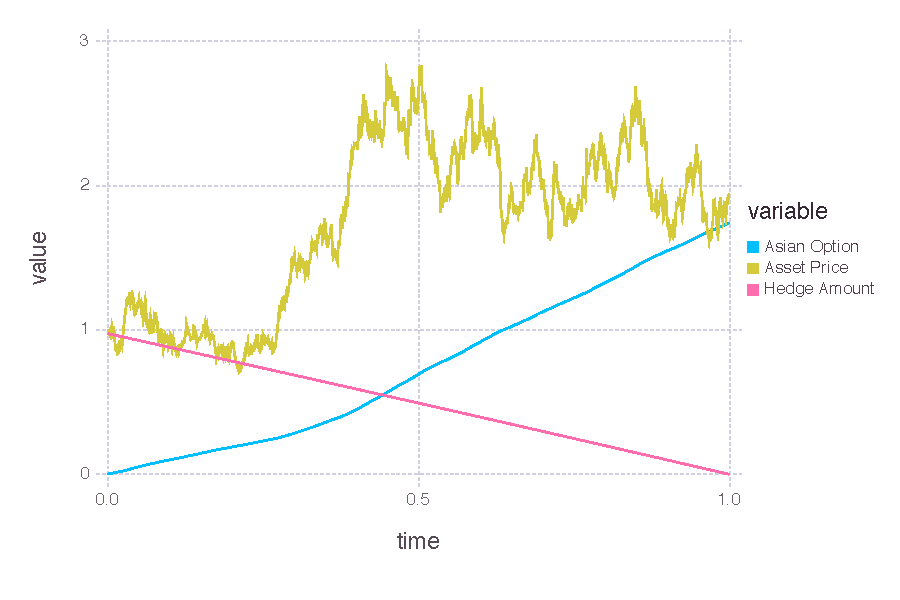
\includegraphics[width=\linewidth]{figures/problemset_1_1.pdf}



\section{Code}

\begin{juliacode}
using Distributions
using Gadfly
using DataFrames

#######################################
# Basic Brownian Motion Functions
#######################################
function make_walk(steps::AbstractArray{Float64,1}, start = 0.0)
    reduce((a,b) -> append!(a, a[end] + b), [start], steps)
end

make_time(N, T) = range(0, T/N, N)
brownian(N, T, start = 0.0) = make_walk(rand(Normal(0, sqrt(T/N)), N-1), start)

geom(w, mu, sigma, t) = exp(sigma*w + (mu - sigma^2/2)*t)
geometric(brownian, time, mu, sigma) = [geom(b,mu,sigma,t) for (b,t) in zip(brownian, time)]

#######################################
# Asians
#######################################

# T/N is like 1/T in discrete
# N - i is like (T - t)
discount(r, N, T, i) = exp(-r * T/N * (N - i))

function expected_value(y, s, r, i, N, T)

    d = discount(r, N, T, i)
    y * T/N * d + s/r * T/N * (1 - d)
end

function asian_value(S, r, N, T)
    Y = cumsum(S)
    [expected_value(Y[i], S[i], r, i, N, T) for i in 1:N]
end

hedge(r, i, N, T) = 1/r * (1 - discount(r, N, T, i))
hedge_value(r, N, T) = [hedge(r, i, N, T) for i in 1:N]

function path_and_price(r, mu, sigma, N, T)
    time = make_time(N, T)
    asset = geometric(brownian(N,T), time, mu, sigma)
    value = asian_value(asset, r, N, T)
    hedge = hedge_value(r, N, T)
    vcat(DataFrame(value = value, time = time, variable = fill("Asian Option", N)),
         DataFrame(value = asset, time = time, variable = fill("Asset Price", N)),
         DataFrame(value = hedge, time = time, variable = fill("Hedge Amount", N)))
end

function plot_asian(r, mu, sigma, N, T)
    d = path_and_price(r, mu, sigma, N, T)
    plot(d, x = :time, y = :value, color = :variable, Geom.line)
end
\end{juliacode}



\end{document}